% Copyright 2026 Torbjörn E. M. Nordling
% SPDX-License-Identifier: Apache-2.0
% frame-step-06.tex — Step to 0.6: the model fits (9:00–11:00)
% Article §3.2: \UpSixFinal, \UpSixGain, \UpSixTau, \UpSixRms, \UpSixNoiseRms,
% \UpSixDelayD, \PredTwo.
\begin{frame}{Step 2: rest to 0.6 --- the first-order model fits}{\dots\ and still contradicts step 1}
  \footnotesize
  \begin{columns}[T]
    \column{0.58\textwidth}
    \centering
    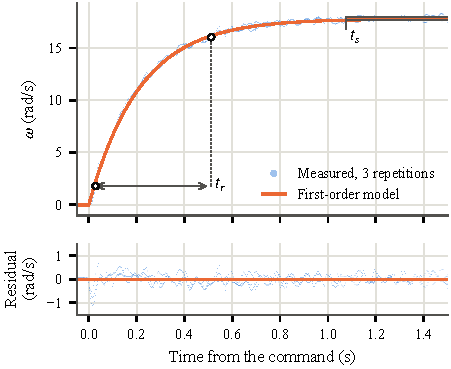
\includegraphics[width=\linewidth, height=0.8\textheight, keepaspectratio]{fig-step-06.pdf}
    \column{0.4\textwidth}
    \scriptsize
    \begin{itemize}\setlength{\itemsep}{3pt}
      \item Final speed \UpSixFinal\,rad/s.
      \item Fit: $G = \UpSixGain$\,rad/s, $\tau = \UpSixTau$\,ms.
      \item RMS error \UpSixRms\,\%, against \UpSixNoiseRms\,\% for the measurement noise alone.
      \item A dead time comes out as $\theta = \UpSixDelayD$\,ms: less than one frame.
      \item But this model predicts \alert{\PredTwo\,rad/s at duty 0.2}, where the wheel stood still.
    \end{itemize}
    \vspace{2pt}
    \alert{A good fit of one step does not show that the system is linear.}
  \end{columns}
\end{frame}
